\documentclass{standalone}
\usepackage{tikz}
\usetikzlibrary{arrows.meta}
\usepackage{tcolorbox}
\usepackage{xcolor}

\definecolor{prismNavy}{HTML}{174A7E}
\definecolor{prismInk}{HTML}{202B36}
\definecolor{prismTeal}{HTML}{007C83}
\definecolor{prismTealLight}{HTML}{D9F0EF}
\definecolor{prismOrange}{HTML}{B85C00}
\definecolor{prismOrangeLight}{HTML}{FFF0D9}
\definecolor{prismGreen}{HTML}{287A3D}
\definecolor{prismGreenLight}{HTML}{E1F2E5}

\begin{document}
\tcbox[
    colback=white,
    colframe=prismNavy,
    arc=4pt,
    boxrule=1.2pt,
    boxsep=2pt,
    left=2pt,
    right=2pt, 
    top=2pt, 
    bottom=2pt
]{%
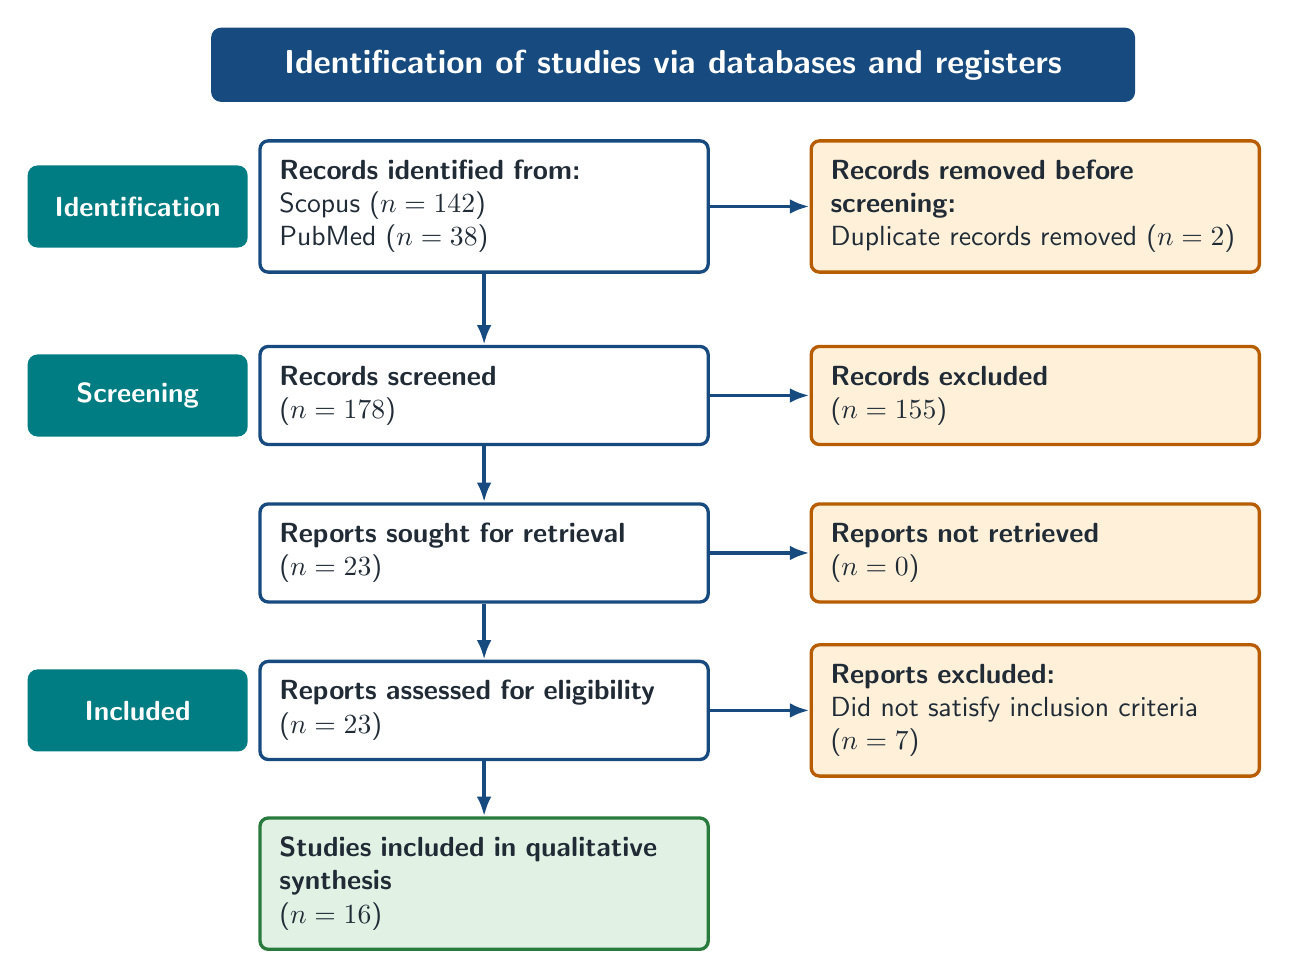
\begin{tikzpicture}[
    font=\sffamily\normalsize,
    box/.style={rectangle, draw=prismNavy, very thick, rounded corners=3pt, align=left, text width=5.2cm, minimum height=1.05cm, inner sep=7pt, fill=white, text=prismInk},
    widebox/.style={rectangle, draw=prismNavy, very thick, rounded corners=3pt, align=center, text width=11.2cm, minimum height=0.9cm, inner sep=7pt, fill=prismNavy, text=white, font=\sffamily\bfseries\large},
    phase/.style={rectangle, draw=prismTeal, very thick, rounded corners=3pt, align=center, text width=2.4cm, minimum height=1.0cm, inner sep=5pt, fill=prismTeal, text=white, font=\sffamily\bfseries},
    arrow/.style={-{Latex[length=2.5mm]}, line width=1.4pt, draw=prismNavy}
]
\node[widebox] (title) at (3.6,0) {\textbf{Identification of studies via databases and registers}};
\node[phase] (identlabel) at (-3.2,-1.8) {Identification};
\node[box] (identified) at (1.2,-1.8) {\textbf{Records identified from:}\\Scopus ($n=142$)\\PubMed ($n=38$)};
\node[box, draw=prismOrange, fill=prismOrangeLight] (removed) at (8.2,-1.8) {\textbf{Records removed before\\screening:}\\Duplicate records removed ($n=2$)};
\node[phase] (screenlabel) at (-3.2,-4.2) {Screening};
\node[box] (screened) at (1.2,-4.2) {\textbf{Records screened}\\($n=178$)};
\node[box, draw=prismOrange, fill=prismOrangeLight] (excluded) at (8.2,-4.2) {\textbf{Records excluded}\\($n=155$)};
\node[box] (sought) at (1.2,-6.2) {\textbf{Reports sought for retrieval}\\($n=23$)};
\node[box, draw=prismOrange, fill=prismOrangeLight] (notretrieved) at (8.2,-6.2) {\textbf{Reports not retrieved}\\($n=0$)};
\node[phase] (includedlabel) at (-3.2,-8.2) {Included};
\node[box] (assessed) at (1.2,-8.2) {\textbf{Reports assessed for eligibility}\\($n=23$)};
\node[box, draw=prismOrange, fill=prismOrangeLight] (reportsexcluded) at (8.2,-8.2) {\textbf{Reports excluded:}\\Did not satisfy inclusion criteria ($n=7$)};
\node[box, draw=prismGreen, fill=prismGreenLight] (included) at (1.2,-10.4) {\textbf{Studies included in qualitative synthesis}\\($n=16$)};
\draw[arrow] (identified) -- (removed);
\draw[arrow] (identified) -- (screened);
\draw[arrow] (screened) -- (excluded);
\draw[arrow] (screened) -- (sought);
\draw[arrow] (sought) -- (notretrieved);
\draw[arrow] (sought) -- (assessed);
\draw[arrow] (assessed) -- (reportsexcluded);
\draw[arrow] (assessed) -- (included);
\end{tikzpicture}%
}%
\end{document}